\chapter{Algorytm rozwiązania}\label{chap:solution_algorithm}

\begin{figure}[H]    
    \centering
    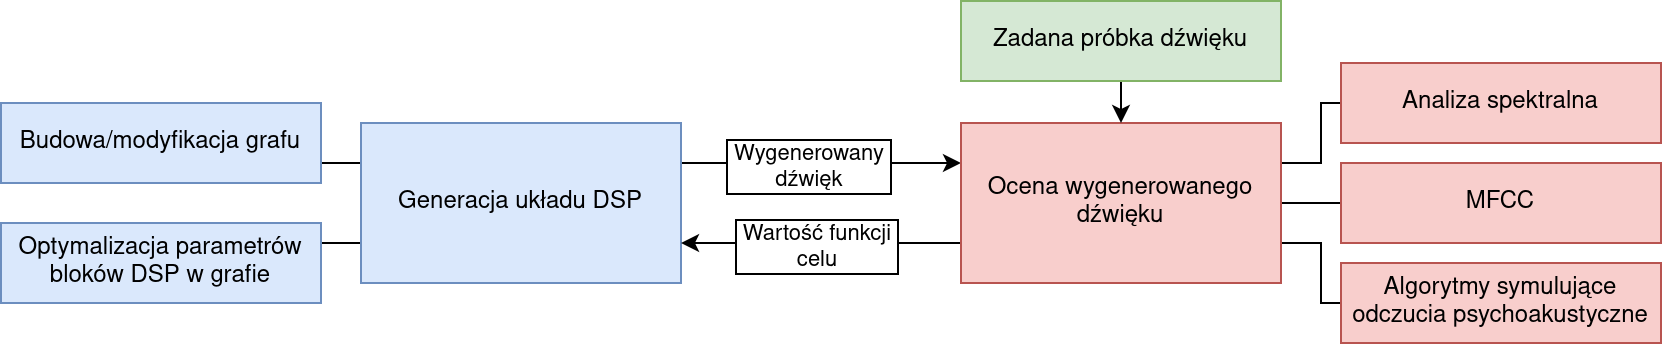
\includegraphics[width=1.0\linewidth]{rys04/solution_algorithm_diagram.png}
    \caption{
      Diagram algorytmu rozwiązania zaimplementowanego w ramach pracy.
      Algorytm oceny może wykorzystywać różne funkcje celu, finalnie zastosowano
      MFCC oraz \textit{dynamic time wrapping},
      proces wyboru funkcji celu opisuje rozdział~\ref{target_function_chapter}.
    }\label{fig:solution_algorithm_diagram}
\end{figure}

Jak opisano w rozdziale poświęconym definicji problemu~(\ref{chap:problem_definition}), praca
rozwiązuje problem budowy grafu DSP z wykorzystaniem dwóch algorytmów:
\begin{enumerate}
  \item Algorytm generujący graf DSP, opisany w rozdziale~\ref{dsp_graph_chapter},
  \item Algorytm oceniający jak bardzo wygenerowany dźwięk jest bliski dźwiękowi docelowemu pod względem barwy,
    opisany w rozdziale~\ref{target_function_chapter}.
\end{enumerate}

Praca wykorzystuje algorytm genetyczny, w którym genotyp odpowiada za strukturę grafu oraz wartości
przypisane do parametrów grafu~(\ref{eq:graph_structure_generation_function},~\ref{eq:graph_params_assignment}).
Diagram blokowy~\ref{fig:solution_algorithm_diagram} ilustruje zaimplementowany algorytm.
